\documentclass[12pt, draft]{beamer}
\usetheme{Darmstadt}

\usepackage[utf8]{inputenc}
\usepackage[german]{babel}
\usepackage[T1]{fontenc}
\usepackage{amsmath}
\usepackage{amsfonts}
\usepackage{amssymb}
\usepackage{tikz}
\usepackage{tabularx}
\usepackage{pgfpages}
\usepackage{listings}
\usepackage{color}

\setbeameroption{show notes on second screen}

\title{Implementation eines Blokus-Spielers}
\author{\mbox{Lukas Jagemann}}
\date{\today}

\lstset{
	aboveskip=1mm,
	belowskip=1mm,
	showstringspaces=false,
	columns=flexible,
	basicstyle={\small\ttfamily},
	numbers=none,
	breaklines=true,
	breakatwhitespace=true,
	tabsize=4
}
% https://tex.stackexchange.com/questions/89574/language-option-supported-in-listings
\lstdefinelanguage{JavaScript}{
	keywords={typeof, new, true, false, catch, function, return, null, catch, switch, var, if, in, while, do, else, case, break},
	keywordstyle=\color{blue}\bfseries,
	ndkeywords={class, export, boolean, throw, implements, import, this},
	ndkeywordstyle=\color{darkgray}\bfseries,
	identifierstyle=\color{black},
	sensitive=false,
	comment=[l]{//},
	morecomment=[s]{/*}{*/},
	commentstyle=\color{purple}\ttfamily,
	stringstyle=\color{red}\ttfamily,
	morestring=[b]',
	morestring=[b]"
}

\begin{document}

\begin{frame}
    \begin{figure}[h]
        \centering
        \resizebox{0.5\linewidth}{!}{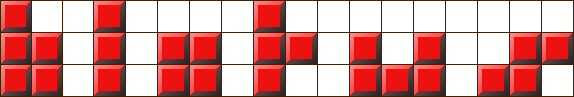
\includegraphics{media/blokus.png}}
    \end{figure}
    %\vspace*{-20pt}
    \titlepage
\end{frame}

\begin{frame}{Inhalt}
	\note{...}
	\setcounter{tocdepth}{1}
    \tableofcontents
\end{frame}

\section{Blokus}
\subsection{Überblick}
\begin{frame}
	Entstanden $\sim$2000\\
	Ursprünglich für 4 Spieler
    \begin{figure}[tp]
        \centering
        \resizebox{0.7\linewidth}{!}{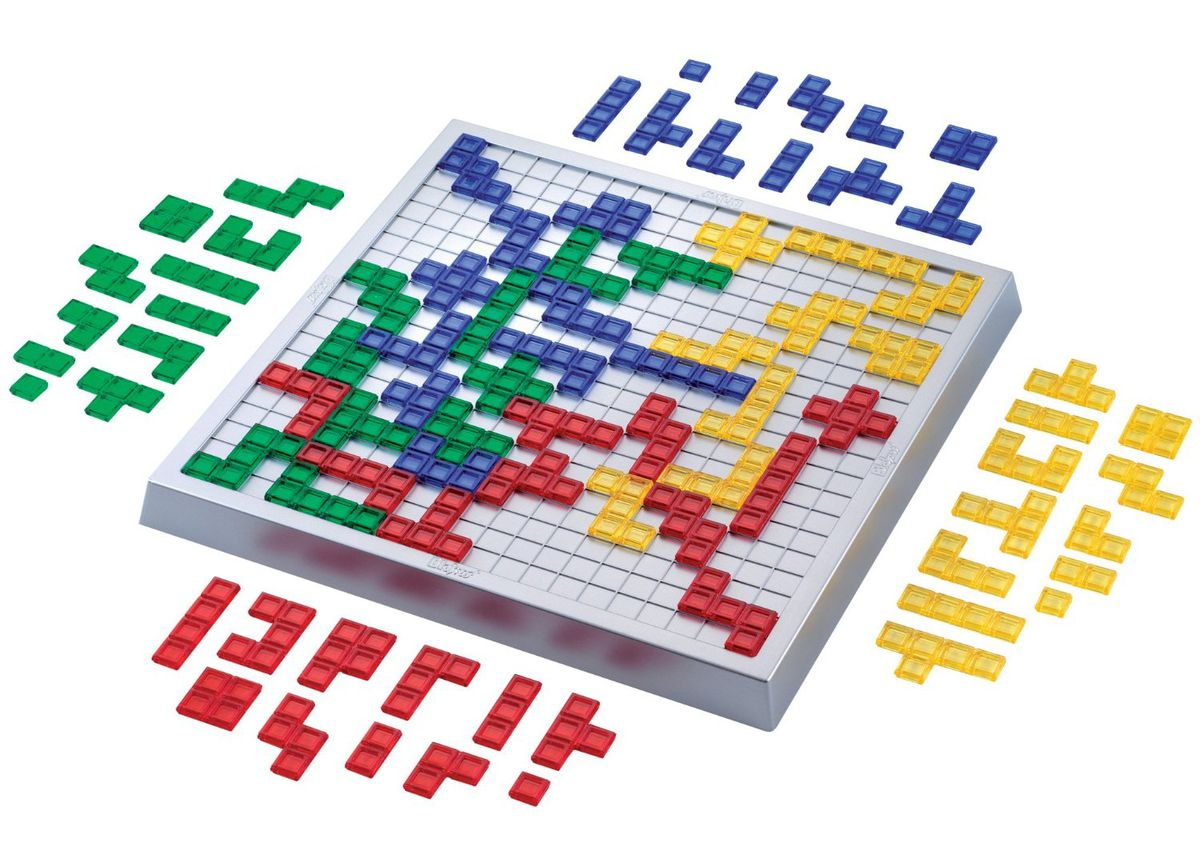
\includegraphics[width=\linewidth]{media/blokus4p.jpg}}\\
        \tiny Quelle: \url{https://media.takealot.com/covers\_tsins/32082437/81LEjjVViUL.\_SL1500\_-zoom.jpg}
    \end{figure}
\end{frame}
\begin{frame}
	\begin{tabularx}{\hsize}{*2{>{\centering\arraybackslash}X}}
		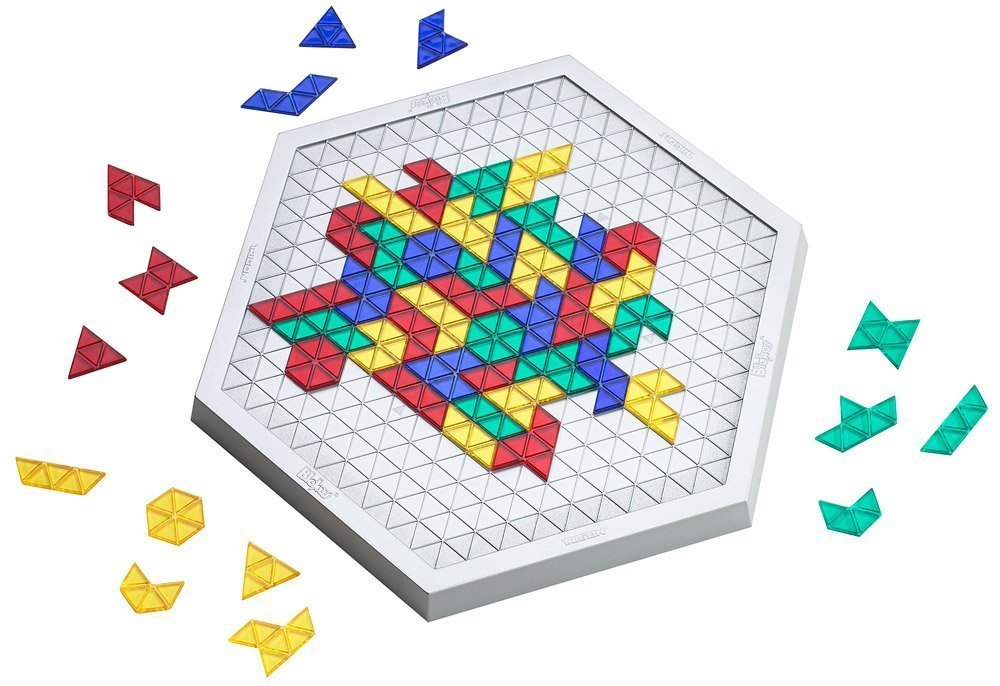
\includegraphics[width=\linewidth]{media/blokus3p.jpg}\linebreak
		\tiny Quelle: \url{http://www.passionforpuzzles.com/weblog/wp-content/uploads/2010/12/613KSlRx9oS._SL1500_.jpg}
	    &
		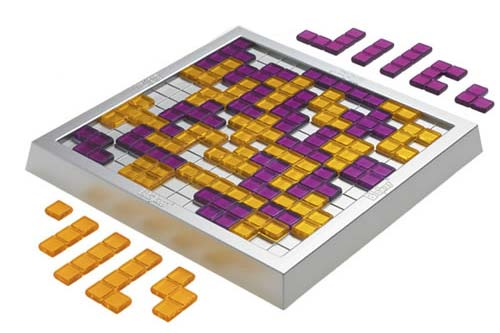
\includegraphics[width=\linewidth]{media/blokus2p.jpg}\linebreak
		\tiny Quelle: \url{http://boardgaming.com/wp-content/uploads/2012/02/blokus-duo-game-in-play.jpg}
	\end{tabularx}
\end{frame}

\subsection{Wie man startet}
\begin{frame}
	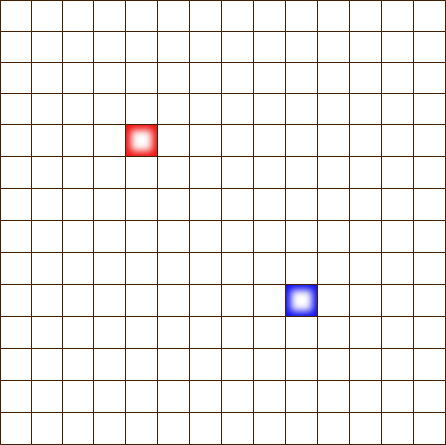
\includegraphics[width=0.8\linewidth]{media/how2play0.png}
\end{frame}
\begin{frame}
	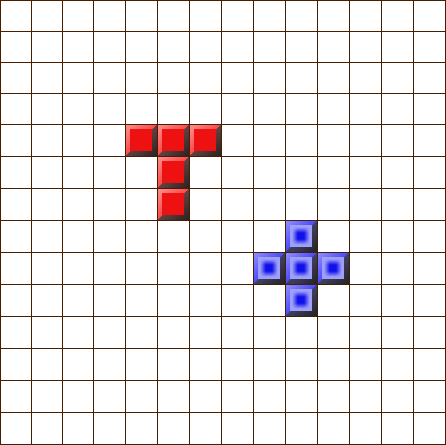
\includegraphics[width=0.8\linewidth]{media/how2play1.png}
\end{frame}

\subsection{Wie man spielt}
\begin{frame}
	\begin{tabular}{c c}
		\huge \color{green} $\checkmark$ & \\
		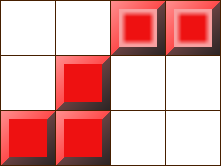
\includegraphics[width=0.5\linewidth]{media/how2play2.png}
		&
	\end{tabular}
\end{frame}
\begin{frame}
	\begin{tabular}{c c}
		\huge \color{green} $\checkmark$ & \huge \color{green} $\checkmark$\\
		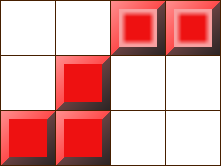
\includegraphics[width=0.5\linewidth]{media/how2play2.png}
		&
		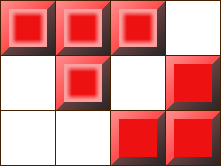
\includegraphics[width=0.5\linewidth]{media/how2play3.png}
	\end{tabular}
\end{frame}
\begin{frame}
\begin{tabular}{c c}
	\huge \color{red} $\times$ & \\
	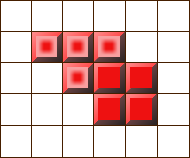
\includegraphics[width=0.5\linewidth]{media/how2play4.png}
	&
\end{tabular}
\end{frame}
\begin{frame}
\begin{tabular}{c c}
	\huge \color{red} $\times$ & \huge \color{green} $\checkmark$\\
	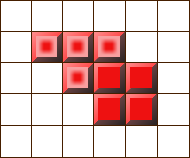
\includegraphics[width=0.5\linewidth]{media/how2play4.png}
	&
	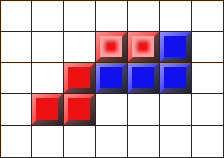
\includegraphics[width=0.5\linewidth]{media/how2play5.png}
\end{tabular}
\end{frame}

\subsection{Wie man gewinnt}
\begin{frame}
	\note{Begriff 'Bits' erklären!}
	Spieler mit den meisten 'Bits' auf dem Feld gewinnt.
	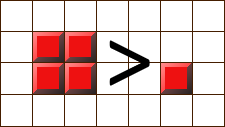
\includegraphics[width=0.7\linewidth]{media/how2play6.png}
\end{frame}

\subsection{Online Ressourcen}
\begin{frame}
	\note{Strategy guter Einstieg\\ Pentolla online spielen. Aktive community!\\Eigenwerbung}
	\begin{itemize}
		\item \url{http://blokusstrategy.com/}
		\item \url{http://pentolla.com/play/}
		\item und jetzt auch: \url{http://splamy.com/blokus/}
	\end{itemize}
\end{frame}


\section{Das Projekt}
\subsection{Wunderschönes CSS3(LESS) und HTML5}
\begin{frame}
	\frametitle{HTML5}
	\begin{itemize}
		\note{Alternative: SVG; Aufwendige Effekte\\Alternative: Canvas2D; Canvas selber zeichnen, Reihenfolge beachten, clickevents selber umrechen\\(ein kandidat mit svg), (einer mit canvas) (zwei plain html)}
		\item Valides HTML5 !
		\item Beste Kompatibilität zwischen aktuellen Browsern
		\item Kurzzeitig Canvas2D, dann doch 'plain' HTML
	\end{itemize}
\end{frame}
\begin{frame}
	\note{Farben in echtzeit änderbar}
	\frametitle{CSS3}
	\begin{itemize}
		\item Einfache hardware-beschleunigte Effekte:\\
			
\includegraphics{media/beautiful0.png}
		\pause
		\item Transformationen und Animationen:
			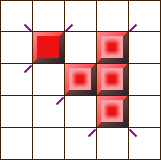
\includegraphics{media/beautiful1.png}
	\end{itemize}
\end{frame}
\begin{frame}
	\frametitle{LESS}
	\note{Alternative SCSS, SASS,...\\Hust, alle Mühen vergebens; Seite sieht trozdem miserabel aus.}
	\begin{itemize}
		\item LESS ist ein CSS precompiler
		\item Praktische Funktionen wie z.B. Variablen und Farbmanipulationen
	\end{itemize}
% TODO vielleicht noch ein Bild hier, aber nicht nötig
\end{frame}

\subsection{TypeScript, das bessere JavaScript}
\begin{frame}[fragile]
	\frametitle{TypeScript}
	\note{JS ist valides TS\\TS starke Empfehlung nicht plain JS zu schreiben\\ES6 implementiert viele TS features\\Verhindert viele allgemeine Fehler\\IDE error support\\IDE syntax vervollständigung\\Einheitliche kompilierung nach ES3, ES5, ES6,...}
	TypeScript...
	\begin{itemize}
		\item ist eine Untermenge von JavaScript
		\item wird transpiliert zu JavaScript
		\item hat Klassen:\\
		\begin{lstlisting}[language=JavaScript]
class A {
	public Prop: boolean;
	private field: number;
}
		\end{lstlisting}
		\item ...mit Vererbung
		\item hat ein strenges Typensystem:\\
		\begin{lstlisting}[language=JavaScript]
let a: boolean = 5; // FEHLER!
		\end{lstlisting}
		\item ...und vieles mehr
	\end{itemize}
\end{frame}

\subsection{Code Struktur}
\begin{frame}
	\begin{itemize}
		\item Modular aufgeteilt in Klassen
		\item Mit Bedacht auf Erweiterbarkeit entworfen:\\ \vspace*{5pt}
			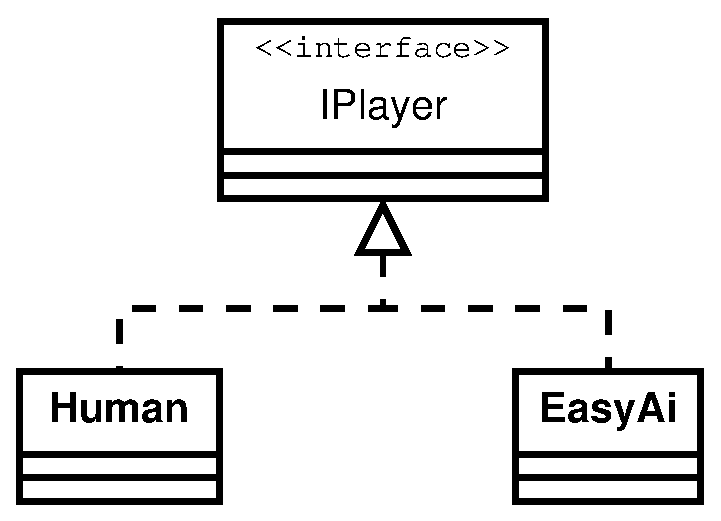
\includegraphics[width=0.5\linewidth]{media/structure1.eps}
	\end{itemize}
\end{frame}
\begin{frame}
	Z.b.\\ \vspace*{5pt}
	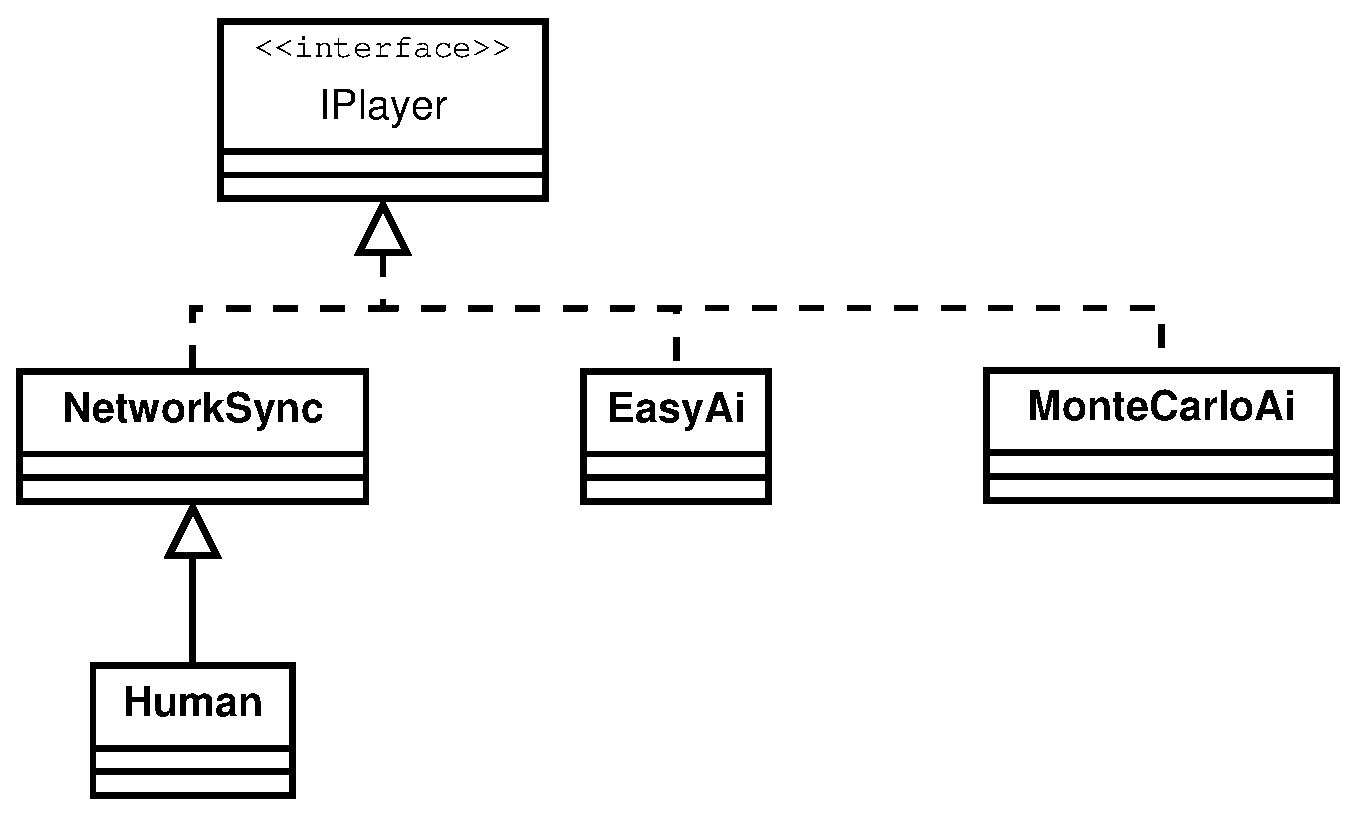
\includegraphics[width=0.8\linewidth]{media/structure2.eps}
\end{frame}

\subsection{GameState}
\begin{frame}
	Ein GameState beschreibt einen kompletten Spielzustand:
	\begin{itemize}
		\item Wer ist dran
		\item Welche Steine sind noch verfügbar
		\item Wie sieht das Spielfeld aus
		\item (Caching)
	\end{itemize}
\end{frame}
\begin{frame}
	\note{=>History slider\\Sehr wichtig beim lernen\\noch wichtiger beim debuggen :P\\Serializierbarkeit}
	Aber warum der Extraaufwand?\\ \vspace*{5pt}
	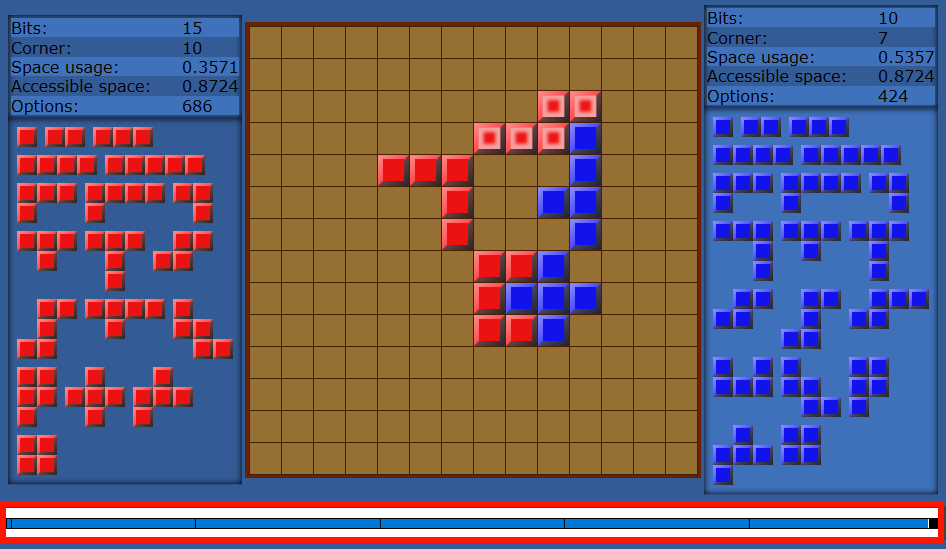
\includegraphics[width=\linewidth]{media/gamestate1.png}
\end{frame}

\section{Minimax}
\subsection{Wie funktioniert MiniMax}
\begin{frame}
	\note{Minimax macht keine riskanten züge\\Für informatiker wachsen Bäume falsch rum :P}
	Eigenschaften von MiniMax:
	\begin{itemize}
		\item basiert darauf das \emph{beide} Spieler optimal spielen
		\item lässt sich rekursiv beliebig stark machen (theoretisch)
		\item spielt 'sicher'
	\end{itemize}
	Wie MiniMax funktioniert:\\
	Für jede Rekursionsstufe wird abwechselnd für einen eigenen Zug die beste und einen gegnerischen Zug die für einen schlechteste Möglichkeit gewählt. Dafür werden die Knoten auf der untersten Ebene ausgewertet und der Baum von unten nach oben reduziert.\\
\end{frame}

% Ziel: beide spieler spielen optimal
\subsection{Grafische Veranschaulichung}
\begin{frame}
\end{frame}

\subsection{Wann MiniMax gut funktioniert}
\begin{frame}
\end{frame}
% Geringes branching
% Berechenbarer status
% (oft gegen ende stark)
\subsection{...und wann eher weniger}
\begin{frame}
\end{frame}
% möglichkeiten graph hier
% hohes branching
% wenig 
\subsection{Abwandlungen}
\begin{frame}
\end{frame}
% aplha beta heuristiken

\section{Die Logik}
\subsection{Konzept}
\begin{frame}
\end{frame}
\subsection{Gewichtung: Bits}
\begin{frame}
\end{frame}
\subsection{Gewichtung: Ecken}
\begin{frame}
\end{frame}
\subsection{Gewichtung: TrueLength}
\begin{frame}
\end{frame}
\subsection{Gewichtung: Weitestes Feld}
\begin{frame}
\end{frame}
\subsection{Gewichtung: Erreichbare Felder}
\begin{frame}
\end{frame}
\subsection{Gewichtung finden}
\begin{frame}
\note{Alles in einen Topf werfen, umrühren, und sich fragen warum die AI genauso schlecht spielt wie vorher!}
\end{frame}
% Selber nachdenken
% Erfahrung
% Problem: Unnormierte Werte
\subsection{...oder finden lassen}
\begin{frame}
\end{frame}
% Genetic failure :P

\section{Optimierungen}
% Javascript...
\subsection{Problem: MiniMax Tiefe?}
\begin{frame}
\end{frame}
% hohe kosten für evaluation
\subsection{Lösung: Adaptiver MiniMax}
\begin{frame}
\end{frame}
% zacken diagramm
\subsection{Berechnungen wiederverwenden}
\begin{frame}
\end{frame}
\subsection{und notfalls löschen}
\begin{frame}
\end{frame}
\subsection{Multithreading (oder so)}
\begin{frame}
\end{frame}
\subsection{Inkrementelle GameStates}
\begin{frame}
\end{frame}

% + alpha/beta

\section{Mögliche Optimierungen (Ausblick)}
\subsection{Kleine Steine am Anfang ignorieren}
\begin{frame}
\end{frame}
\subsection{Dynamische Gewichtung}
\begin{frame}
\end{frame}
\subsection{Summen-Erreichbare Felder}
\begin{frame}
\end{frame}
% bla
% =======
\subsection{Anderer Algorithmus?}
\begin{frame}
\end{frame}
% Bild mit den zwei einsern
% Monte carlo ?
% sehr stark heuristik basierend
\subsection{Priorisieren von Gebieten in MiniMax}
\begin{frame}
\end{frame}
% Mehr Rechenleistung in interessante Gebiete stecken
\subsection{Neuschreiben, in einer besseren Sprache}
\begin{frame}
\end{frame}
% Performance, Memorymanagemenet, Threads

\end{document}